Las oscilaciones son perpendiculares a la dirección del movimiento de la onda. En otras palabras, la dirección del movimiento de las oscilaciones y el de la onda ocurre en ejes distintos. Este tipo de onda puede ser \mecanica\ o \electromagnetica.

\begin{figure}[H]
  \centering
  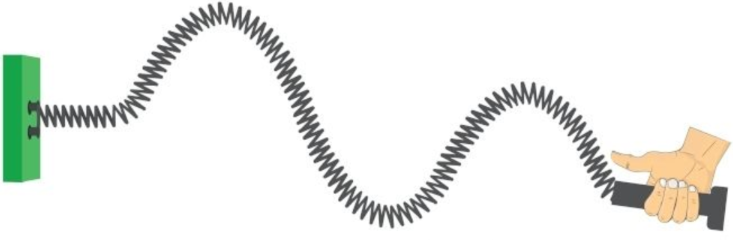
\includegraphics[scale=0.4]{imagenes/onda_transversal.png}
  \caption{Onda transversal\cite{educacao}}
\end{figure}

Ejemplos:

\begin{itemize}
  \item Ondas de radio.
  \item Luz visible.
  \item Rayos gamma.
  \item Ondas en un resorte.
\end{itemize}
